\chapter{Stacks and Queues}

Stacks and queues are data structures, adapted from our daily lives. We realized that we can implement stacks and queues using arrays or linked lists. We will look at the concept on how to implement them efficiently (All of their operations should be done in $O(1)$ time, that is constant time regardless of size.) and write C++ code for the array implementation\footnote{As mentioned in Chapter 5 it is difficult to code the linked list implementation in C++, hence we will not do so in this chapter and also the upcoming chapters, however, an intuition will be given on how to do so potentially}.

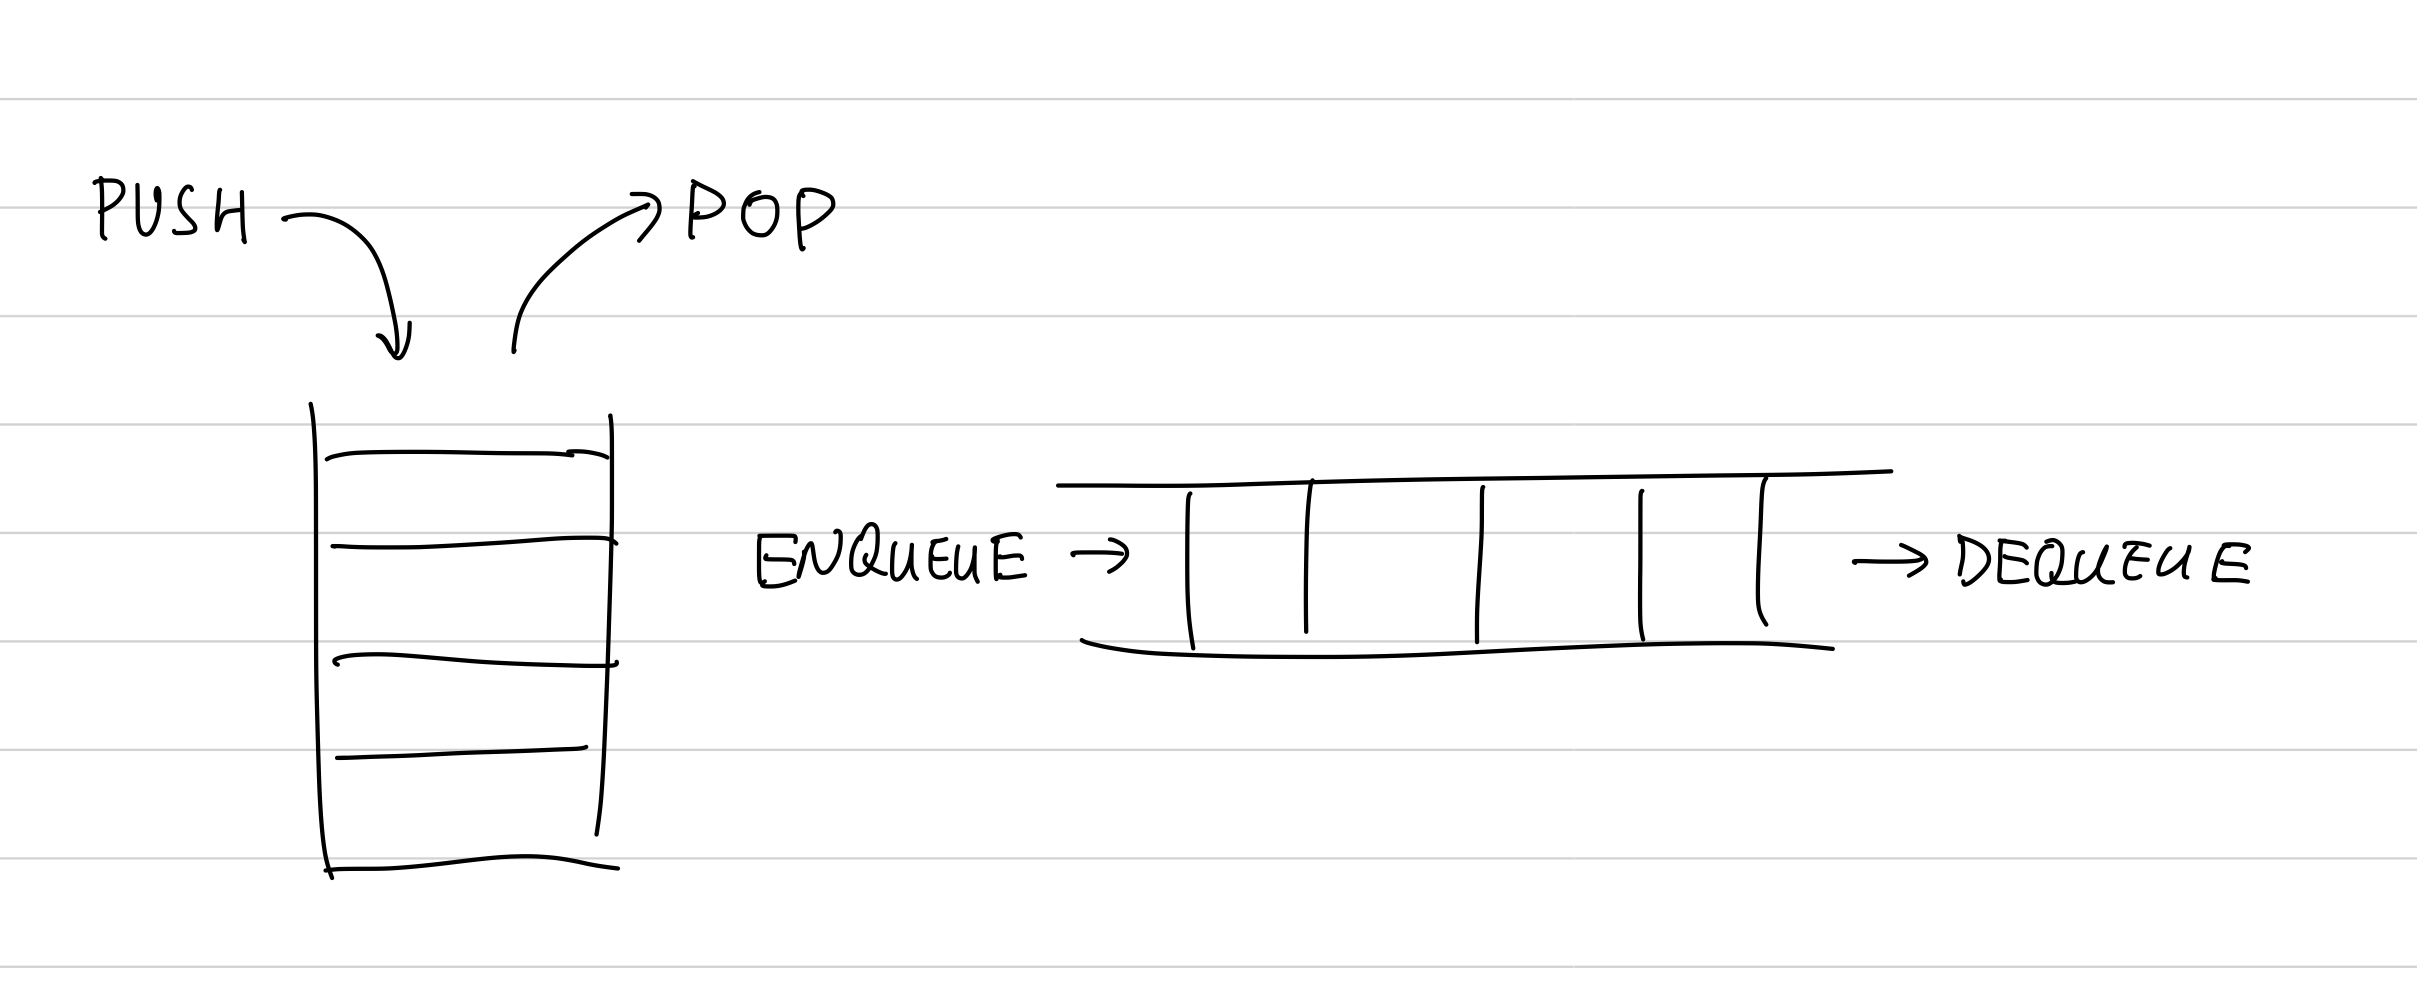
\includegraphics[width=15cm]{images/ch6-stackqueue.png}

\section{Stack}
Say you have a stack of towels put in a box, you would probably first use the towels on top, and you would also put new washed towels on the top. This is a stack, elements can only be inserted and removed at one end, what we call, last in first out (LIFO)\index{last in first out (LIFO)}.

\begin{table}[h]
    \centering
    \begin{tabular}{|m{11em}|m{24em}|}
        \hline
        \textbf{Operations of a stack} & 
        Usage
        \\ \hline \hline
        
        \texttt{void push(int x)}\tablefootnote{It can store any other data types other than integers, however integer is selected for easier understanding, same applies to a lot of the algorithms discussed in the coming chapters} &
        Insert \texttt{x} to the top of the stack.
        \\ \hline
        
        \texttt{int pop()} &
        Remove the element at the top of the stack, and return value of the removed element.
        \\ \hline
        
        \texttt{bool isEmpty()} &
        Returns \texttt{true} when the stack is empty, \texttt{false} otherwise.
        \\ \hline
        
        \texttt{int size()} &
        Return the current number of elements in the stack.
        \\ \hline
    \end{tabular}
\end{table}

Stacks can be easily implemented by both arrays and linked lists. As demonstrated by the illustrations. 

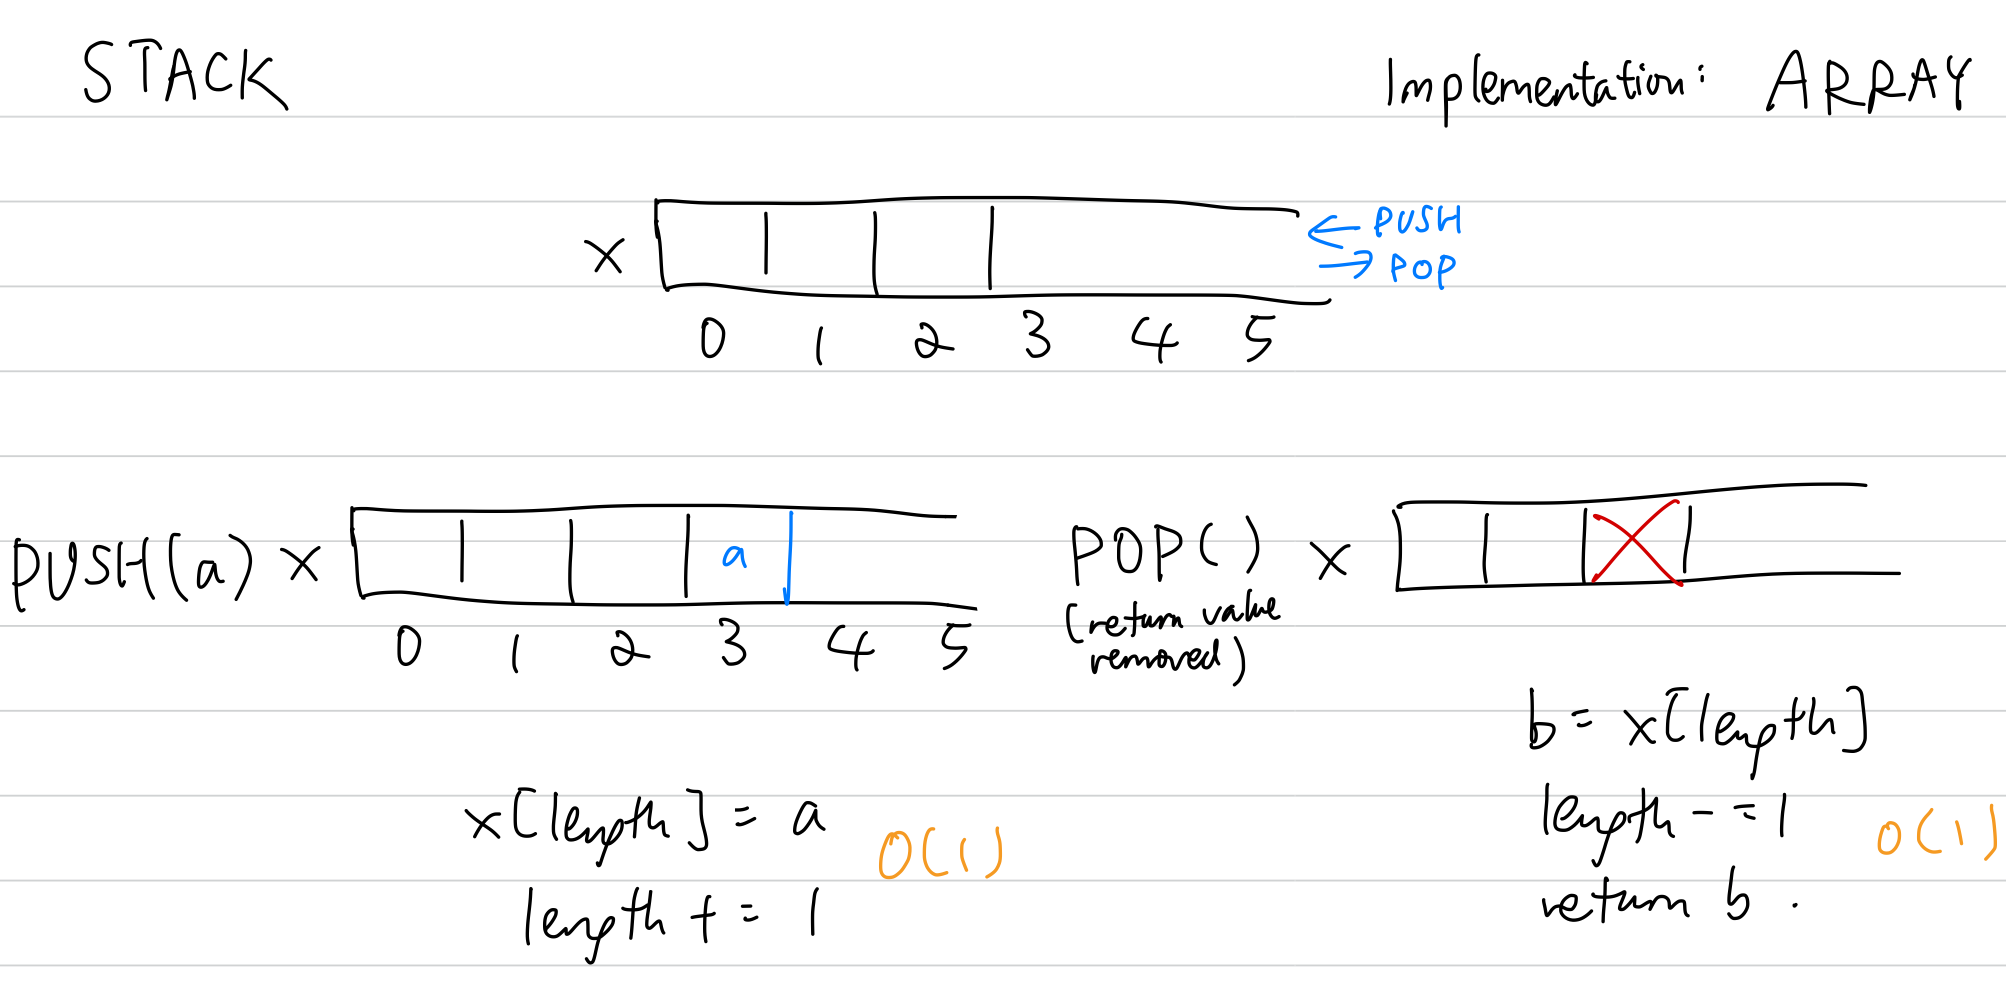
\includegraphics[width=15cm]{images/ch6-stackarray.png}

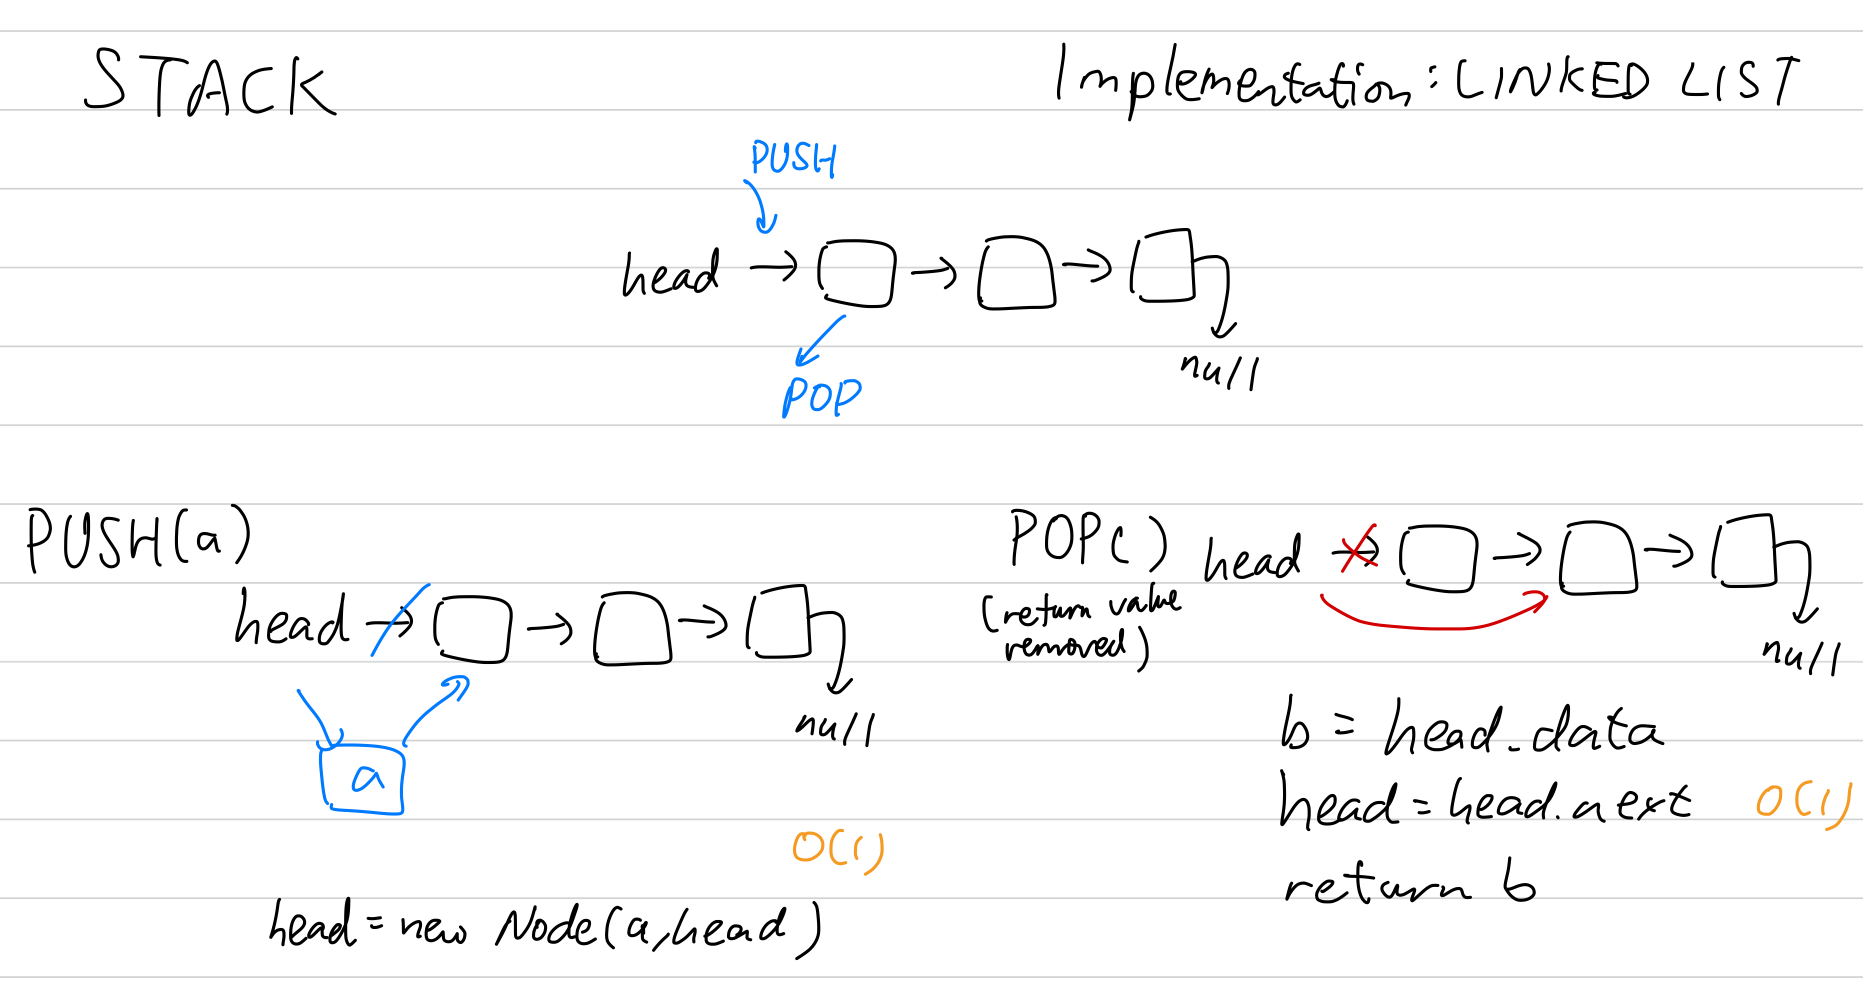
\includegraphics[width=15cm]{images/ch6-stacklinkedlist.png}

Let's look at the array implementation in code. In the illustrations, we assumed that the array have an infinite size. In reality, array memory is limited, so we impose a MAX value and stop pushing elements when the stack is full.
\vspace{6mm}

C++: (\textit{Exercise: Try to re-implement yourself.})\footnote{The way to deal with the warnings when the stack is full/ empty depends on the use case. We will not cover it here.}
\begin{lstlisting}
const int MAX = 20; //can be larger
int stk[MAX] = {}; //declare new empty array of size MAX
int _size = 0;

void push(int x){
    if(_size==MAX){ //what would happen if we remove this check?
        cout << "WARNING: Stack is full." << endl;
        return;
    }
    stk[_size] = x;
    _size++;
}

int pop(){
    if(_size==0){ //what would happen if we remove this check?
        cout << "WARNING: Stack is empty." << endl;
        return -1;
    }
    int x = stk[_size];
    _size--;
    return x;

    //alternatively: (less intuitive)
    // _size--;
    // return stk[_size+1];
}

int size(){ return _size;}

//Can we check whether the stack is empty by if(pop()==-1) instead?
bool isEmpty(){ return _size==0;}
\end{lstlisting}

Use example:
\begin{lstlisting}
int main(){
    cout << size() << " " << isEmpty() << endl; //0 1
    push(4);
    cout << size() << " " << isEmpty() << endl; //1 0
    push(5);
    cout << size() << " " << isEmpty() << endl; //2 0
    cout << pop() << endl; //5
    cout << size() << " " << isEmpty() << endl; //1 0
    cout << pop() << endl; //4
    cout << size() << " " << isEmpty() << endl; //0 1
    pop(); //WARNING: Stack is empty.
    cout << size() << " " << isEmpty() << endl; //0 1
} 
\end{lstlisting}
\section{Queue}
Just like a normal queue in daily life, people queue at one end and they are served when they reach the other end, what we call first in first out (FIFO)\index{first in first out (FIFO)}.

\begin{table}[h]
    \centering
    \begin{tabular}{|m{11em}|m{24em}|}
        \hline
        \textbf{Operations of a queue} & 
        Usage
        \\ \hline \hline
        
        \texttt{void enqueue(int x)} &
        Insert \texttt{x} to one end of the queue.
        \\ \hline
        
        \texttt{int dequeue()} &
        Remove the element at the other end of the queue, and return value of the removed element.
        \\ \hline
        
        \texttt{bool isEmpty()} &
        Returns \texttt{true} when the queue is empty, \texttt{false} otherwise.
        \\ \hline
        
        \texttt{int size()} &
        Return the current number of elements in the queue.
        \\ \hline
    \end{tabular}
\end{table}

Queues can be easily implemented by both arrays and linked lists.

Let's first focus on the array implementation:

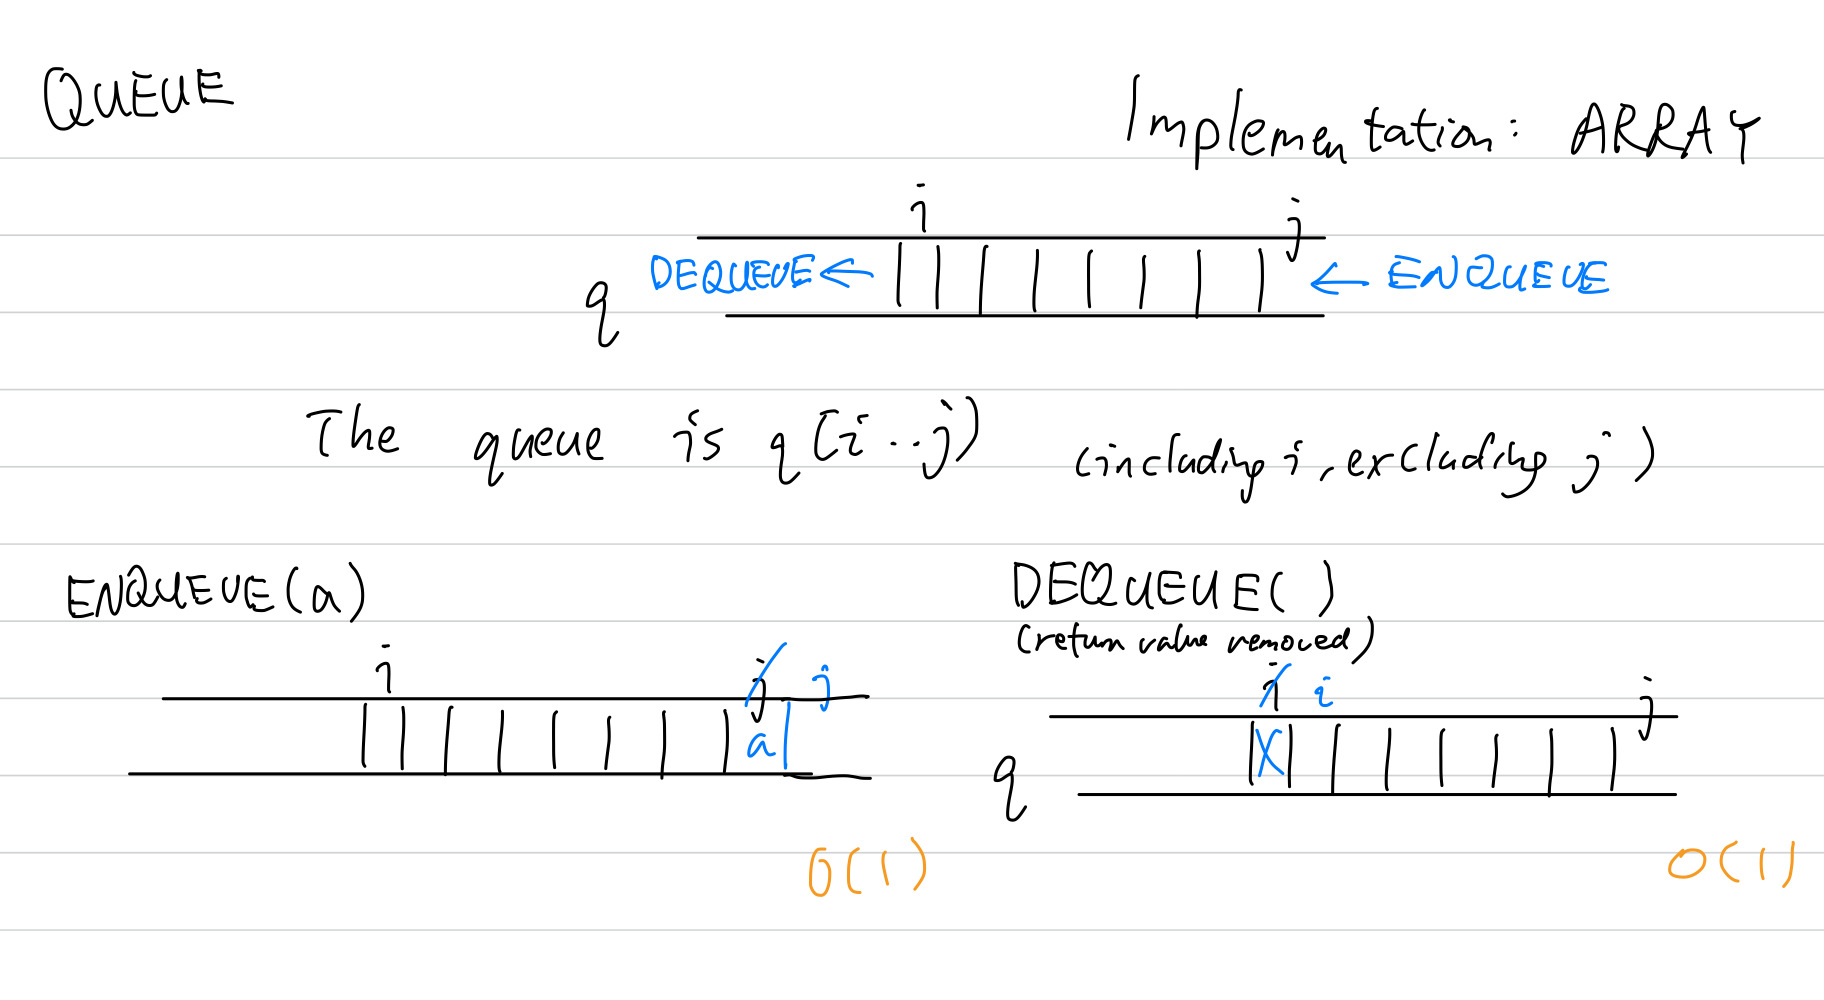
\includegraphics[width=14cm]{images/ch6-qarray.png}

Here is an implementation: \textit{(NOT the one you should follow)}

\begin{lstlisting}
//global variables, can be used by all functions
const int MAX = 20; //constants, cannot be changed throughout the program
int q[MAX] = {};
int i = 0;
int j = 0;
//The queue: q[i..j)

void enqueue(int x){
    if(j==MAX){
        cout << "WARNING: Queue is full." << endl;
        return;
    }
    q[j] = x;
    j++;
}

int dequeue(){
    if(i==j){
        cout << "WARNING: Queue is empty." << endl;
        return -1;
    }
    int x = q[i];
    i++;
    return x;
}

int size(){ return j-i;}

bool isEmpty(){ return i==j;}
\end{lstlisting}

Example usage:

\begin{lstlisting}
int main(){
    cout << size() << " " << isEmpty() << endl; //0 1
    enqueue(4);
    cout << size() << " " << isEmpty() << endl; //1 0
    enqueue(5);
    cout << size() << " " << isEmpty() << endl; //2 0
    cout << dequeue() << endl; //4
    cout << size() << " " << isEmpty() << endl; //1 0
    cout << dequeue() << endl; //5
    cout << size() << " " << isEmpty() << endl; //0 1
    dequeue(); //WARNING: Queue is empty.
    cout << size() << " " << isEmpty() << endl; //0 1
}
\end{lstlisting}

\subsection{Circular queues}

\textit{Difficult topic}
\vspace{6mm}

You can quickly see that there is a problem, variables \texttt{i} and \texttt{j} keep increasing but never decrease, eventually the queue cannot be used after \texttt{MAX} amount of insertions. This is unsustainable and we realized we can work around it.
\vspace{6mm}

The solution is a \textbf{circular queue}\index{circular queue}. Value of variables \texttt{i} and \texttt{j} circle round and round, going back to 0 after reaching \texttt{MAX-1}.

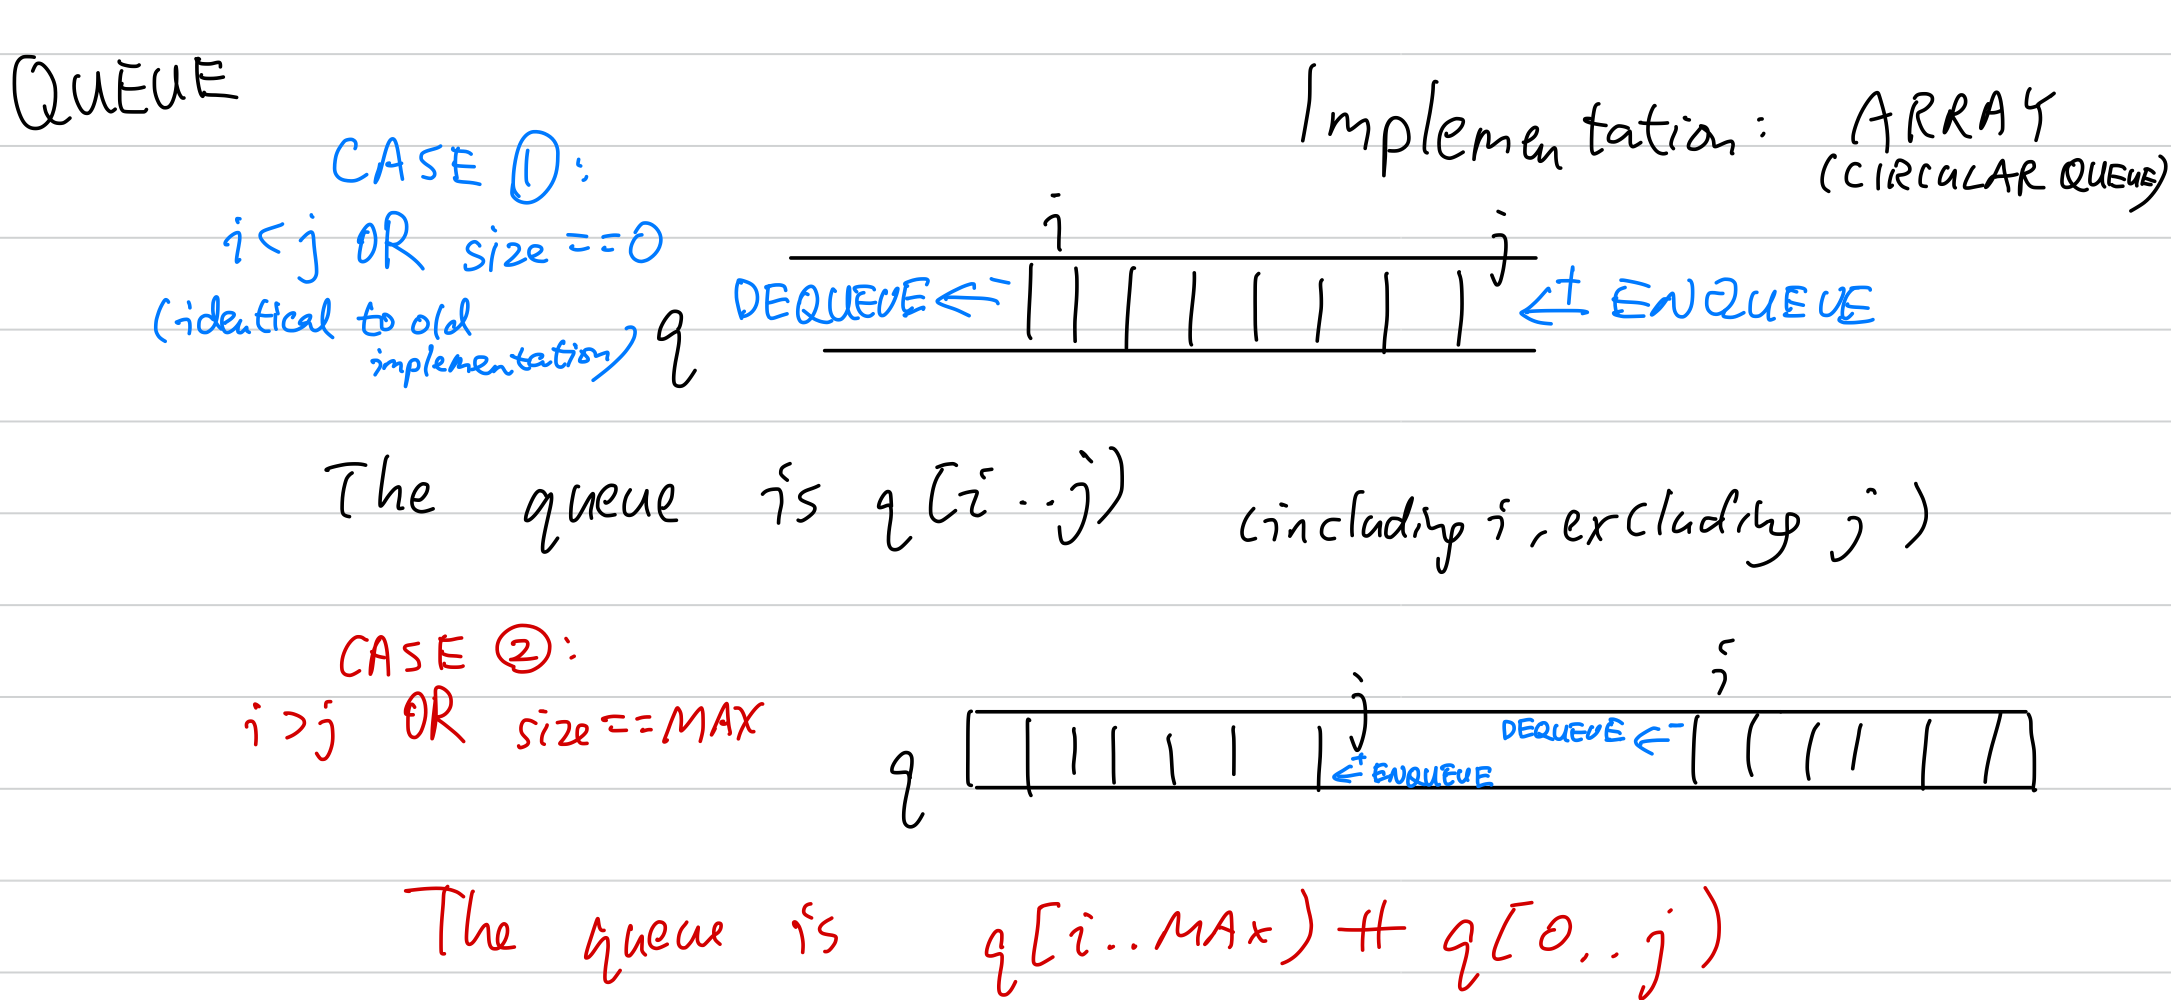
\includegraphics[width=15cm]{images/ch6-cq.png}

There is an ambiguity when \texttt{i=j}, it can either mean the queue is completely full, or the queue is completely empty. One solution is to introduce a \texttt{size} variable, to keep track of the size and differentiate the two cases.

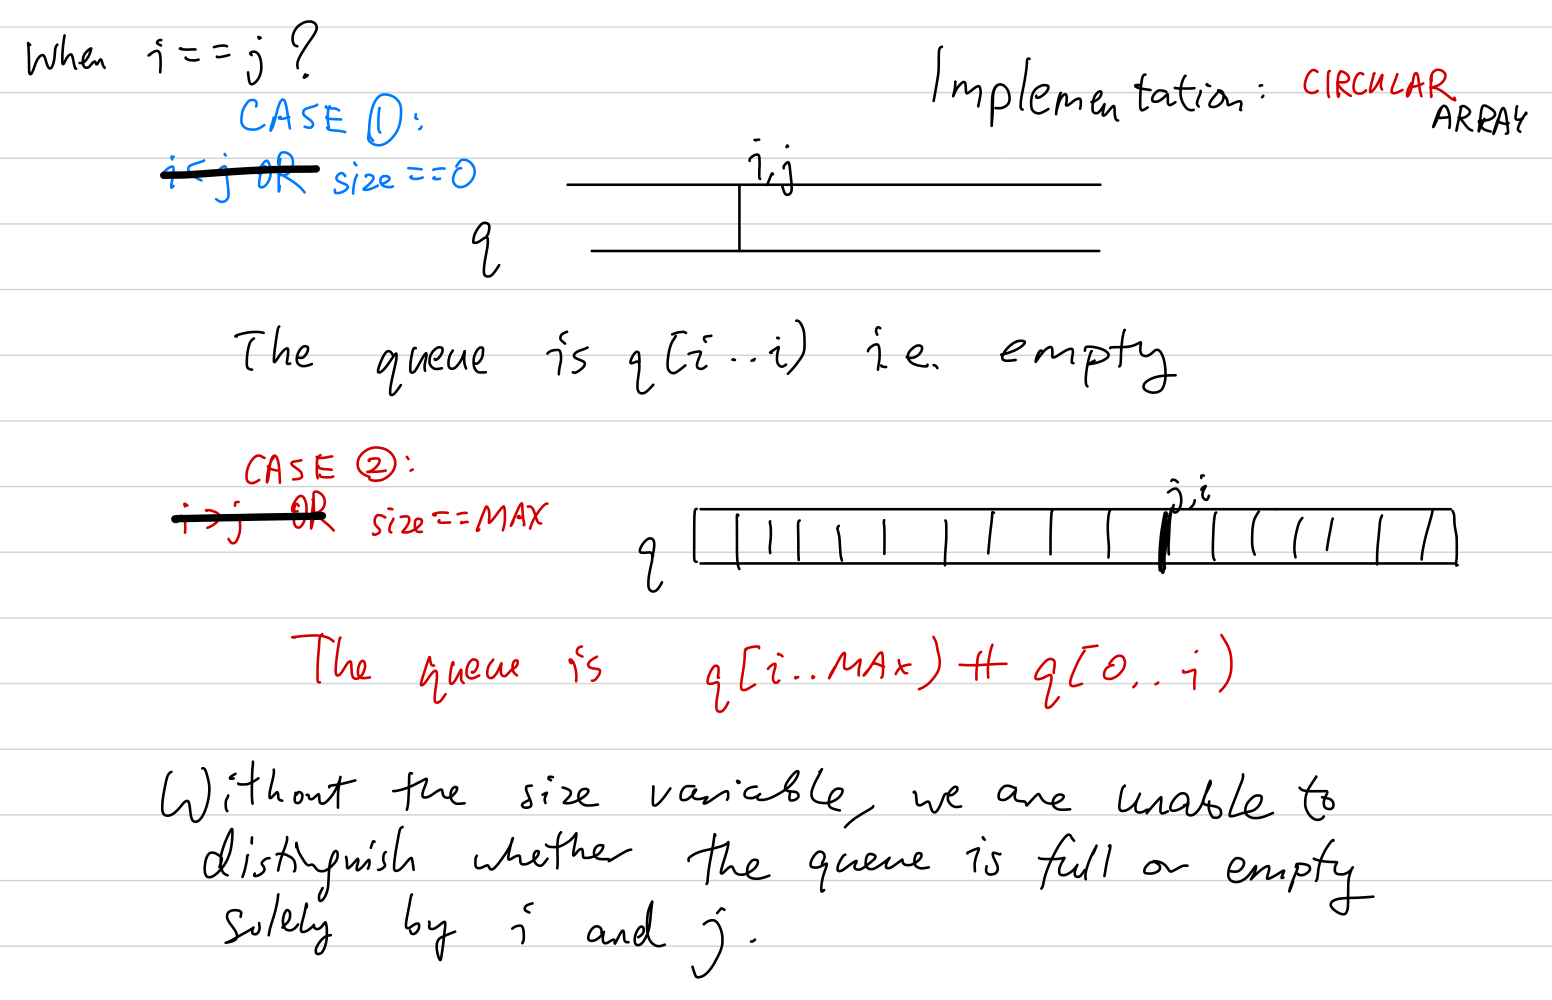
\includegraphics[width=15cm]{images/ch6-cqij.png}

C++: \textit{(Exercise:  Try to re-implement yourself.)}

\begin{lstlisting}
const int MAX = 20; 
int cq[MAX] = {};
int i = 0;
int j = 0;
int _size = 0;

void enqueue(int x){
    if(_size==MAX){
        cout << "WARNING: Queue is full." << endl;
        return;
    }
    cq[j] = x;
    j = (j+1)%MAX; //cycles back to 0 after MAX-1
    _size++;
}

int dequeue(){
    if(_size==0){
        cout << "WARNING: Queue is empty." << endl;
        return -1;
    }
    int x = cq[i];
    i = (i+1)%MAX; //cycles back to 0 after MAX-1
    _size--;
    return x;
}

int size(){ return _size;}

bool isEmpty(){ return _size==0;}
\end{lstlisting}
\vspace{6mm}

Finally, the outline of the linked list implementation is as follows. An additional tail pointer is used so that both enqueue and dequeue can be done in $O(1)$ time.

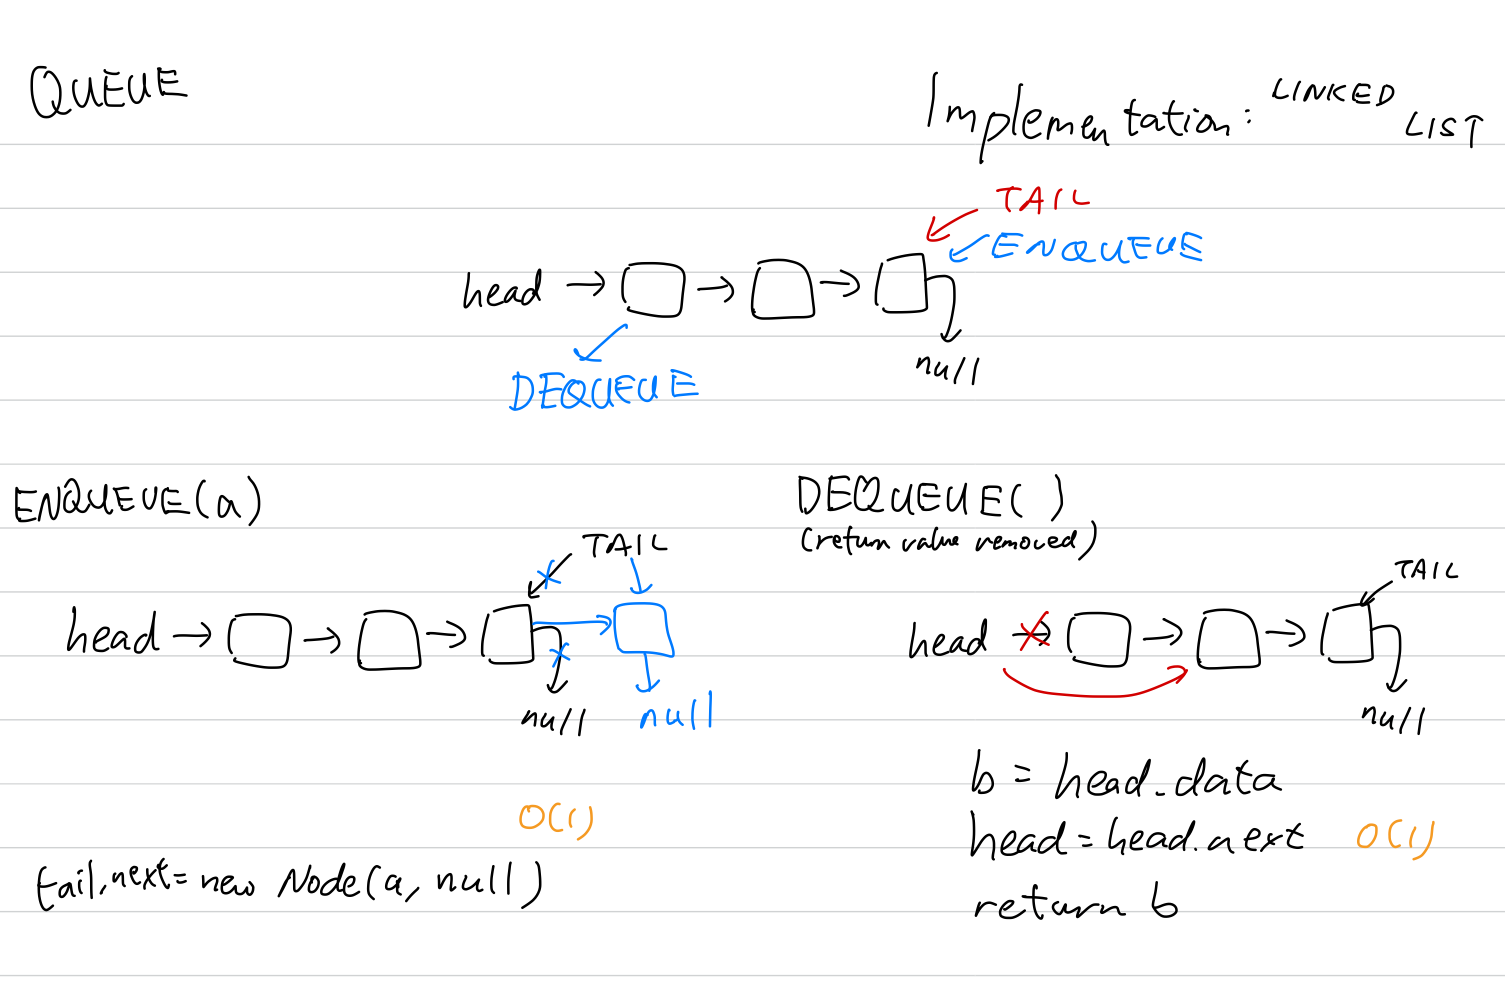
\includegraphics[width=15cm]{images/ch6-qlinkedlist.png}